%% $RCSfile: proj_report_outline.tex,v $
%% $Revision: 1.3 $
%% $Date: 2016/06/10 03:41:54 $
%% $Author: kevin $

\documentclass[11pt
              , a4paper
              , twoside
              , openright
              ]{report}


\usepackage{float} % lets you have non-floating floats

\usepackage{url} % for typesetting urls

\usepackage{tikz}
\usepackage{amsmath}
\usepackage{algorithm}
\usepackage{algpseudocode}
\usepackage{hyperref}
\usepackage{float}

\usepackage{tabularx} % Add this to the preamble

%
%  We don't want figures to float so we define
%
\newfloat{fig}{thp}{lof}[chapter]
\floatname{fig}{Figure}

%% These are standard LaTeX definitions for the document
%%                            
\title{Reinforcement Learning}
\author{James Thompson}

%% This file can be used for creating a wide range of reports
%%  across various Schools
%%
%% Set up some things, mostly for the front page, for your specific document
%
% Current options are:
% [ecs|msor|sms]          Which school you are in.
%                         (msor option retained for reproducing old data)
% [bschonscomp|mcompsci]  Which degree you are doing
%                          You can also specify any other degree by name
%                          (see below)
% [font|image]            Use a font or an image for the VUW logo
%                          The font option will only work on ECS systems
%
\usepackage[font,ecs]{vuwproject}

% You should specifiy your supervisor here with
%     \supervisor{Firstname Lastname}
% use \supervisors if there is more than one supervisor
\supervisor{Dr Aaron Chen}

% Unless you've used the bschonscomp or mcompsci
%  options above use
%   \otherdegree{OTHER DEGREE OR DIPLOMA NAME}
% here to specify degree
\otherdegree{Master of Artificial Intelligence}

% Comment this out if you want the date printed.
\date{\today}

\begin{document}

% Make the page numbering roman, until after the contents, etc.
\frontmatter

%%%%%%%%%%%%%%%%%%%%%%%%%%%%%%%%%%%%%%%%%%%%%%%%%%%%%%%

%%%%%%%%%%%%%%%%%%%%%%%%%%%%%%%%%%%%%%%%%%%%%%%%%%%%%%%

\begin{abstract}

This is submitted for the completion of AIML440 Directed individual study as part of the Master of Artificial Intelligence programme at Victoria University of Wellington. This reports will have three sections. Firstly an Introduction of reinforcement learning and basic algorithms. Secondly I will evaluate modern algorithms. Lastly I will describe a new algorithm and compare it to the state of the art models.

\end{abstract}

%%%%%%%%%%%%%%%%%%%%%%%%%%%%%%%%%%%%%%%%%%%%%%%%%%%%%%%

\maketitle

% Removed because I have no acknowledgements
% \include{acknowledge}

\tableofcontents

% we want a list of the figures we defined
\listof{fig}{Figures}

%%%%%%%%%%%%%%%%%%%%%%%%%%%%%%%%%%%%%%%%%%%%%%%%%%%%%%%

\mainmatter

%%%%%%%%%%%%%%%%%%%%%%%%%%%%%%%%%%%%%%%%%%%%%%%%%%%%%%%

% individual chapters included here

\chapter{Introduction}\label{C:intro}

\subsection{The reinforcement learning problem}

Reinforcement learning is a framework of learning that describes how an agent learns by interacting with the environment. The framework involves 2 entities the agent and environment. The agent is only entity that we as designers have direct control of. We decide how its learns and decides on its actions. The environment is the context and situation that the agent is in. There are three important flows of information;  the state of the environment to the agent, the action decision to the environment and lastly the reward to the agent. This can be best be understood in the figure below.

\begin{fig}
\begin{center}
    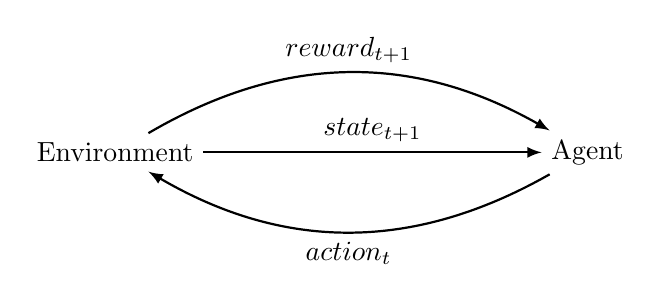
\begin{tikzpicture}[
        node distance=6cm, % Increased node distance for better spacing
    ]
        % Define nodes
        \node (env) {Environment};
        \node (agent) [right of=env] {Agent};

        % Define arrows and labels without boxes
        \draw [-latex,bend left, thick] (env) edge node[anchor=south] {$reward_{t+1}$} (agent);
        \draw [-latex, thick] (env) -- node[anchor=south] {$state_{t+1}$} (agent);
        \draw [-latex,bend left,thick] (agent) edge node[anchor=north] {$action_{t}$} (env);
    \end{tikzpicture}
    \caption{The flow of information between th environment and agent}
\end{center}
\end{fig}

The state is a representation of the information within the environment that the agent will use to make its decision on which action to take. The reward signal is treated as the final word on how good the situation is, the more reward the better, always. Lastly the action is sent to the environment and the environment will in turn return the next state that the action has taken the agent. This brings us to the reinforcement learning problem which can be framed as such "How does the agent decide which actions to take given the state such that it maximises the future cumulative reward". It is important that the agent maximises all *future cumulative* reward otherwise short term gains could be made to the sacrifice of larger long term gains. This idea has been formalised by Richard Sutton as the reward hypothesis

\begin{quote}
    "That all of what we mean by goals and purposes can be well thought of as maximization of the expected value of the cumulative sum of a received scalar signal (reward)." 
    \cite{suttonReinforcementLearningSecond2018}
\end{quote}

\subsection{Formalism}

The reinforcement problem can be formalised as a Markov Decision Process. The MDP is a collection of states, actions and rewards along with a transition function which states that probability of the next reward and state given a state and reward.
$$
Pr\left\{ S_{t}=s', R_{t}=r | S_{t-1}=s, A_{t-1}=a \right\} 
$$
This function completely characterises the dynamics of the environment. This abstraction of the environment to a MDP is widely applicable and serves as the basis for much of reinforcement learning.  We can see here that transition function only looks at the previous state. It can do this because we assume that the state representation has the *Markov property* [@suttonReinforcementLearningSecond2018], which states including previous states in the conditional wont change the probability as the current state will have already captured that information. In interaction with the agent the MDP will generate a sequence that looks like:
$$S_{1},A_{1},R_{2},\dots S_{n},A_{n}, R_{n+1},\dots$$
In the case above we have an infinite sequence and these are continuing tasks as they have no end. Alternatively you could have episodic tasks that have a start and ending with a terminal state.
"The cumulative sum of a received scalar signal" part of the reward hypothesis can be formalised to be the return $G$.
$$
G_{t}=R_{t+1}+\gamma R_{t+2}+\gamma^{2}R_{t+3}\dots=\sum_{k=t}^{\infty}\gamma^{t-1}R_{t+1}
$$

$\gamma$ is called the discounting factor. It is usually added for two reasons. Firstly because it means that the return won't be infinite which simplifies it mathematically. Secondly is due to the very natural intuition that the future is less predicable than the present, thus more distance rewards should have less weight as they are less certain. 


A decision agent will use policy $\pi$ which provides the probability of taking action $a$ given state $s$. This policy could be deterministic or stochastic.
To get the policy the agent needs an understanding of value of its current state. This is called the value function and it is a expectation of the future rewards.
$$
v_{\pi}(s)=\mathbb{E}\left[ G_{t}| S_{t}=s\right] 
$$
The value function depends on the state, policy and discounting factor $\gamma$. In a similar vain to value function we have the action-value function which is the expected future reward given a state and action taken.

$$
q_{\pi}(s,a) = \mathbb{E}\left[ G_{t} | S_{t}=s, A_{t}=a \right] 
$$

These functions are closely related and have a large amount of connected definitions this one:

$$
q_{\pi}(s,a)=\mathbb{E}\left[ R_{t+1}+\gamma v_{\pi}(S_{t+1})|S_{t}=s, A_{t}=a \right] 
$$

The maximising part of the reinforcement problem can be solved by the finding optimal actions. We can define both $v_{\star}=\underset{ \pi }{ \text{max} }\ v_{\pi}(s)$ and $q_{\star}=\underset{ \pi }{ \text{max} }\ q_{\pi}(s,a)$ as the optimal value given optimal actions afterwards.
If we can find $q_{\star}$ then the problem is solved as we could make a policy $\pi_{\star}$ that is greedy with respect to $q_{\star}$. 

This form explicitly learning a value function then implicitly getting a full policy or just needed actions from it is called value based methods. Alternatively you can learn the policy directly with policy based methods. The effectiveness of these methods depend heavily on how easy the value function or policy is to learn.

\chapter{Algorithms}\label{C:algorithms}

In the real world we don't get access to the transition function of the MDP. The agents only method to learn is through interacting with the environment. From this interaction we get a sample of the environment and must learn from it. Therefore stochastic learning methods must be used. Two learning ideas are core for many reinforcement learning algorithms. These are Monte Carlo \cite{suttonReinforcementLearningSecond2018} and Temporal Difference learning \cite{suttonTemporalCreditAssignment1984} \cite{suttonLearningPredictMethods1988}.

\subsection{Traditional algorithms}

Monte Carlo learning works by estimating the value function as being the average return from that state.  A basic algorithm would look like this.

\begin{algorithm}
\caption{Monte Carlo Control with Exploring Starts}
\begin{algorithmic}[1]
\State Arbitrarily initialize $\pi(s) \in \mathcal{A}(s)$ and $Q(s,a) \in \mathbb{R}$
\State $\text{Returns}(S,A) \gets$ empty list
\For{each episode}
    \State Arbitrarily choose $S_0 \in \mathcal{S}, A_0 \in \mathcal{A}$
    \State Generate an episode by following $\pi$
    \State $G \gets 0$
    \For{each step of the episode $t = T-1, T-2, \dots, 0$}
        \State $G \gets \gamma G + R_{t+1}$
        \If{$(S_t, A_t)$ does not appear earlier in the episode}
            \State Append $G$ to $\text{Returns}(S_t, A_t)$
            \State $Q(S_t, A_t) \gets \text{average}(\text{Returns}(S_t, A_t))$
            \State $\pi(S_t) \gets \arg\max_{a} Q(S_t, a)$
        \EndIf
    \EndFor
\EndFor
\end{algorithmic}
\end{algorithm}

Because we need a well defined return Monte Carlo methods only work on episodic tasks. It will only update the states that it actually visits, therefore it has the advantage that we can force it to explore just the state space we are interested in, by starting it in states we want to know about.

Temporal difference learning works different incrementally updating the value of a state with the received reward and the value of the next state. As the update is using its own estimate it is *bootstrapping*. Because of this bootstrapping it can work with both episodic and continuing environments.

\begin{equation}
V(S_{t})=R_{t+1}+\gamma V(S_{t+1})
\end{equation}

Below is a basic implementation of TD learning for a continuing environment, however one can see how you could easily make it just go on forever in an continuing environment.

\begin{algorithm}
\caption{TD(0)}
\begin{algorithmic}[1]
\State Initialize $Q(s,a)$ arbitrarily and set $Q(\text{terminal-state}) = 0$
\State Initialize $S$
\While{not converged}
    \State Take action $A$, observe $R$, $S'$
    \State Choose $A' \in \mathcal{A}(S')$ using policy derived from $Q$
    \State $Q(S,A) \gets Q(S,A) + \alpha \left[ R + \gamma Q(S', A') - Q(S,A) \right]$
    \State $S \gets S'$; $A \gets A'$
\EndWhile
\end{algorithmic}
\end{algorithm}

This particular update is known as TD(0) because it only looks one step into the future. However it can be generalised to be TD(n). One can see that if we had TD($\infty$) we would be back at Monte Carlo

The two methods of TD(n) and Monte carlo can be to get the best of both worlds using TD($\lambda$) methods \cite{suttonLearningPredictMethods1988}.

There are two issues with the Naive methods of TD and Monte Carlo methods mentioned above. This is scalability and exploration.

Firstly with scalability we are storing the action value of a particular state in a large lookup table. This will immediately become a problem when dealing with large state or action spaces. Most real world application have tremendously large state/action spaces. Furthermore it is easy to imagine how most of the states have overlapping information and are actually really quite similar. Therefore instead of learning $Q$ directly we can try and learn an appropriator $\hat{Q}$.

Second problem is exploration. As we learn we are finding better and better actions. These better action are taken which will form our trajectory. What can happen here is that we miss large chunks of the state space. To solve this we can instead use a sub optimal policy that deliberately takes exploratory actions. $\epsilon$-greedy is a good example of this as it will take a random action with probability $\epsilon$ and an optimal action the rest of the time. Alternatively you can use a different exploration policy to interact with the environment while you are learning the optimal. This method of learning from experience using a different policy is called off-policy learning. The previous methods we looked at are both on-policy.

\subsection{Modern Deep learning algorithms}\label{sec:MDLA}

\subsubsection{Deep Q Networks}
\label{subsec:DQN}

One can take the TD(0) learning algorithm and apply the notion of off-policy learning we get SARSAMAX otherwise known as Q-Learning \cite{watkinsLearningDelayedReward1989} \cite{watkinsQlearning1992} . It works almost the same except the action value function is updated using the best possible action taken at the next state.

\begin{equation}
Q(S_{t}, A_{t}) \leftarrow Q(S_{t}, A_{t}) + \alpha \left( R_{t+1}+\gamma \max_{a} Q(S_{t+1}, a) - Q(S_{t}, A_{t}) \right) 
\end{equation}

As with TD(0) this fails when faced with a sufficiently large state and/or action space. To resolve this we can use a function approximator, which means we no longer need to store a mapping for every single state. The most powerful function approximators we have are neural networks \cite{hornikMultilayerFeedforwardNetworks1989}. Therefore we can apply a neural network as an approximator $\hat{Q}$ for $Q$. The algorithm we get is called Deep-Q-Learning \cite{mnihPlayingAtariDeep2013}\cite{mnihHumanlevelControlDeep2015}. It was applied very successfully to match and exceed human level performance on a large variety of Atari 2600 games (Space invaders, pong etc).

Here is the algorithm that Mnih et al used in their papers \cite{mnihPlayingAtariDeep2013} \cite{mnihHumanlevelControlDeep2015}.

\begin{algorithm}
\caption{Deep Q-Learning (DQN)}
\begin{algorithmic}[1]
\State Initialize replay memory $D$ with capacity $N$
\State Initialize action-value function $Q$ with random weights $\theta$
\State Initialize target action-value function $\hat{Q}$ with weights $\theta^{-} = 0$
\For{episode = 1 to $M$}
    \State Initialize sequence $s_{1} = \{ x_{1} \}$ and preprocessed sequence $\phi_{1} = \phi(s_{1})$
    \For{$t = 1$ to $T$}
        \State With probability $\epsilon$, select a random action $a_{t}$
        \State Otherwise, select $a_{t} = \arg\max\limits_{a} Q(\phi(s_{t}), a; \theta)$
        \State Observe reward $r_{t}$ and next state $x_{t+1}$
        \State Set $s_{t+1} = (s_{t}, a_{t}, x_{t+1})$ and preprocess $\phi_{t+1} = \phi(s_{t+1})$
        \State Store transition $(\phi_{t}, a_{t}, r_{t}, \phi_{t+1})$ in $D$
        \State Sample random minibatch of transitions $(\phi_{j}, a_{j}, r_{j}, \phi_{j+1})$ from $D$
        \State Set $\gamma_{j} \gets$
        \[
        \begin{cases} 
        r_j, & \text{if episode terminates at step } j+1 \\
        r_{j} + \gamma \max\limits_{a'} \hat{Q}(\phi_{j+1}, a'; \theta^{-}), & \text{otherwise}
        \end{cases}
        \]
        \State Perform a gradient descent step on 
        \[
        \left( \gamma_{j} - Q(\phi_{j}, a_{j}; \theta) \right)^{2}
        \]
        \State Every $C$ steps, reset $\hat{Q} \gets Q$
    \EndFor
\EndFor
\end{algorithmic}
\end{algorithm}

There are more features of this algorithm that are different than traditional Q-learning. These are important to solve problems the arise when you add a neural network approximator into the learning process of Q-learning.

The first of these ideas is called experience replay \cite{10.5555/168871}, which is collecting your experience in a replay memory $D$. Then to learn you can loop through your experience and extract as much as you can from your previous experiences. The idea in Deep Q-learning is that at each time step rather than updating $\hat{Q}$ with your current experience you update it using a sampled transition from $D$. This helps with an important problem which is that stochastic gradient descent assumes independent and identically distributed data (**i.i.d**). As experience is collected each transition will be dependent on the previous transition and will affect the next transition thus the independent assumption is not held. Thus randomly sampling from $D$ will give you a independent data set. This also makes DQN a off policy learning method

The second assumption is that the training data is identically distributed. Gradient descent is working towards the target $\gamma$. The problem is that the target involves our current prediction, so as we learn a better prediction our target will move. This results in a chase which decreases learning efficiency. The solution to this as seen in the algorithm is fixing $\hat{Q}$ for a fixed number of steps $C$. It uses $\hat{Q}$ in the target $\gamma_{j}$ but then updates $Q$ every $C$ updates. This gives the network a reasonable opportunity to tend towards the target $\gamma_{j}$ while still using a recent estimate of the action value.

Lastly is the concept of pre-processing the state to speed up the learning process. One can decrease the computational complexity of the neural network by simplifying the state using a transformation that in theory doesn't lose the meaningful information. Minh et al used this in their 2013 paper to make the video input; smaller, conform to the ratio their model needed and making it gray scale. We can see that this pre-processing step is the only example of domain specific knowledge that would be needed for an implementation of the algorithm to a task.

\subsubsection{Soft Actor-Critic}\label{subsec:SAC}

The DQN method discussed above, along with TD and MC learning, are all value-based methods. That is, they learn to evaluate how good a current situation is (whether that be a state or state-action), and then a policy can be generated by maximizing over the value function. Another approach is to directly learn the policy function. A combination of these ideas leads to the actor-critic framework.

In an actor-critic framework, there is a policy that controls how the agent acts, $\pi$, as well as a value function that evaluates how good the action taken was. A good way to update the policy is based on whether the result was better or worse than what the critic expected. Using the TD error of the critic for this is called A2C \cite{mnihAsynchronousMethodsDeep2016}.

However, there are still challenges in expanding A2C to high-dimensional continuous control tasks. Many current methods are difficult to stabilize and require carefully tuned hyperparameters. To address this, several improvements can be introduced to the actor-critic framework, resulting in Soft Actor-Critic (SAC) \cite{haarnojaSoftActorCriticOffPolicy2018}.

First, similar to DQN \cite{mnihPlayingAtariDeep2013, mnihHumanlevelControlDeep2015}, making it off-policy allows for much better sampling efficiency as more information is extracted from experience. More importantly, SAC employs entropy maximization. Traditional RL agents aim to maximize the expected sum of rewards. However, the maximum entropy RL framework modifies this objective to maximize both the expected reward and the entropy of the policy, leading to the following objective function:

\begin{equation}
J(\pi) = \sum_{t=0}^{T} \mathbb{E}_{(s_{t}, a_{t}) \sim \rho_{\pi}} \left[ r(s_{t}, a_{t}) + \alpha \mathcal{H}(\pi(\cdot|s_{t})) \right] 
\end{equation}

This entropy term encourages exploration, with the temperature parameter $\alpha$ determining the strength of this encouragement. Initially a hyperparameter in \cite{haarnojaSoftActorCriticOffPolicy2018}, the SAC algorithm was later modified to learn and adjust $\alpha$ throughout training \cite{haarnojaSoftActorCriticAlgorithms2019}. This not only improves efficiency—since choosing an optimal temperature is task-dependent and non-trivial \cite{haarnojaSoftActorCriticAlgorithms2019}—but also allows the policy to explore uncertain regions while being more exploitative in familiar areas.

The final SAC algorithm \cite{haarnojaSoftActorCriticAlgorithms2019} is as follows:

\begin{algorithm}[H]
\caption{Soft Actor-Critic Algorithm}
\begin{algorithmic}[1]
\State \textbf{Input:} $\theta_{1}, \theta_{2}, \phi$
\State $\bar{\theta_{1}} \gets \theta_{1}, \bar{\theta_{2}} \gets \theta_{2}$
\State $\mathcal{D} \gets \emptyset$
\For{each iteration}
    \For{each environment step}
        \State Sample action: $a_{t} \sim \pi_{\phi}(a_{t} | s_{t})$
        \State Sample next state: $s_{t+1} \sim p(s_{t+1} | s_{t}, a_{t})$
        \State Store transition: $\mathcal{D} \gets \mathcal{D} \cup (s_{t}, a_{t}, r(s_{t}, a_{t}), s_{t+1})$
    \EndFor
    \For{each gradient step}
        \State Update Q-functions: $\theta_{i} \gets \theta_{i} - \lambda_{Q} \hat{\nabla}_{\theta_{i}} J_{Q}(\theta_{i})$ for $i \in \{1,2\}$
        \State Update policy: $\phi \gets \phi - \lambda_{\pi} \hat{\nabla}_{\phi} J_{\pi}(\phi)$
        \State Update entropy coefficient: $\alpha \gets \alpha - \lambda \hat{\nabla}_{\alpha} J(\alpha)$
        \State Update target Q-networks: $\bar{\theta_{i}} \gets \tau\theta_{i} + (1 - \tau) \bar{\theta_{i}}$ for $i \in \{1,2\}$
    \EndFor
\EndFor
\State \textbf{Output:} $\theta_{1}, \theta_{2}, \phi$
\end{algorithmic}
\end{algorithm}

One noteworthy difference from conventional actor-critic methods is that SAC uses two Q-functions. While not strictly necessary, this significantly speeds up training \cite{haarnojaSoftActorCriticAlgorithms2019}.

Between 2018 and 2019, when SAC was first introduced, it outperformed other popular methods such as TD3 \cite{fujimotoAddressingFunctionApproximation2018}, DDPG \cite{lillicrapContinuousControlDeep2019}, and PPO \cite{schulmanProximalPolicyOptimization2017} in continuous control benchmarks.

\subsubsection{Proximal Polixy Optimizatin}\label{subsec:PPO}

One of the problems that can happen with policy changes is that a small change which results in a different actions being taken can have large consequences. A natural idea is to try and limit the changes that can happen to policy at any step. You can do this by using a surrogate objective function that is limited to be at least somewhat similar to the current policy. This was first implemented using a trust region (i.e an area that we can safely move the policy and is guranteed to improve) and resulted in the TRPO algorithm \cite{schulmanTrustRegionPolicy2017}. Yet the most popular method is that of PPO \cite{schulmanProximalPolicyOptimization2017}, as it is computationally simpler. The method used in PPO is to use a clipped objective which results in a loss function like so:
$$
L^{\text{CLIP}}(s,a,\theta_k,\theta) = \min\left(
\frac{\pi_{\theta}(a|s)}{\pi_{\theta_k}(a|s)}  A^{\pi_{\theta_k}}(s,a), \;\;
\text{clip}\left(\frac{\pi_{\theta}(a|s)}{\pi_{\theta_k}(a|s)}, 1 - \epsilon, 1+\epsilon \right) A^{\pi_{\theta_k}}(s,a)
\right)
$$

Where the advantage function ($A^{\pi_{\theta_{k}}}(s,a)$) is a way of measuring how much better the situation is than expected. The ratio $\frac{\pi_{\theta}(a|s)}{\pi_{\theta_{k}}(a|s)}$ is used to measure the difference between the current policy and the old policy. This ratio is what is clipped and used as a scalar for the advantage function. As we see in the situation that the action was better ($A>0$) the clip function will apply and make sure that $L$ wont be too large, however it can be as small as 0. In the other case when things were worse than expected ($A < 0$) it capped to make $L$ not close to zero (note that $L$ will be negative), yet $L$ could be as large (in the negative sense) as it would like. The reasoning is that allowing for these large and negative $L$ means that we can do a better job of making sure that this action is not taken again.

The advantage function can be can be estimated in many ways . A simple advantage function could be actual return - estimated return ($G_{t} - V(s_{t})$) for episodic tasks, or TD error ($r_{t}+\gamma V(s_{t+1})-V(s_{t})$) for continuing tasks. The implementation in the paper use generalised advantage estimation which is an exponentially weighted sum of TD errors \cite{schulmanHighDimensionalContinuousControl2015}, as it better balances bias and variance. GAE is defined as:

$$
\hat{A_{t}}^{GAE(\gamma, \lambda)} = \sum_{t=0}^{\infty}(\gamma\lambda)^{l}\delta_{t+l}^{V}
$$
Where $\delta_{t}^{V}=r_{t}+\gamma V(s_{t}+1)-V(s_{t})$. $\gamma$ is the usual discounting factor but this is expanded on with $\lambda$ which is from 0-1, at 0 it is TD(0) error and at 1 would be the full complete return.

With this advantage estimator we need to learn a value function. This puts PPO in the same style of actor-critic methods. It is however regarded as a Policy gradient method starting with the author Schulman designating it so.

The CLIP loss function can be augmented with other objectives to increase its effectiveness. For example using entropy maximisation to encourage exploring like what is done above with \ref{subsec:SAC}. This leads to this objective:
$$
L^{\text{CLIP} + S}(s, a, \theta_{k, }\theta)=\hat{\mathbb{E}}_{t}\left[ L^{\text{CLIP}}(s,a, \theta_{k, }\theta)+cS\left[ \pi_{\theta}\right](s)  \right] 
$$
Where $S$ is the entropy of the policy. There is a large space of exploring different surrogate objective functions which incorporate the CLIP function.

Here is a reference version of the algorithm from Open AI's spinning up documentation \cite{openaiProximalPolicyOptimization2020}:

\begin{algorithm}
\caption{PPO Algorithm}
\begin{algorithmic}[1]
\State \textbf{Input:} initial policy parameters $\theta_{0}$, initial value function parameters $\phi_{0}$
\For{$k = 0, 1, 2, \dots$}
    \State Collect set of trajectories $\mathcal{D}_{k} = \{\tau_{i}\}$ by running policy $\pi_{k} = \pi(\theta_{k})$ in the environment.
    \State Compute rewards to go $\hat{R}_{t}$ (This is an estimate of the return $R_{t}$ for each state in the trajectories)
    \State Compute advantage estimates $\hat{A}_{t}$ (using any method of advantage estimation) based on the current value function $V_{\phi_{k}}$
    \State Update the policy by maximizing the PPO-CLIP objective:
    $$
    \theta_{k+1} = \arg \max_{\theta} \frac{1}{|\mathcal{D}_{k}|T}\sum_{\tau \in  \mathcal{D}_{k}} \sum_{t=0}^{T} \min \left( \frac{\pi_{\theta}(a_{t}|s_{t})}{\pi_{\theta_{k}}(a_{t}|s_{t})} A^{\pi_{\theta_{k}}}(s_{t}, a_{t}), \text{clip} \left( \frac{\pi_{\theta}(a_{t}|s_{t})}{\pi_{\theta_{k}}(a_{t}|s_{t})}, 1-\epsilon, 1+\epsilon  \right) A^{\pi_{\theta_{k}}}  \right)
    $$
    \State Fit value function by regression on mean-squared error:
    $$
    \phi_{k+1} = \arg \min_{\phi} \frac{1}{|\mathcal{D}_{k}|T}\sum_{\tau \in  \mathcal{D}_{k}} \sum_{t=0}^{T} (V_{\phi}(s_{t})-\hat{R}_{t})^{2}
    $$
\EndFor
\end{algorithmic}
\end{algorithm}

\chapter{Conclusions}\label{C:con}

\section{Further work}

Finite time and resources have limited the scope of this report. There are many areas that could be explored further. I will outline some of the areas that I would have liked to explore further and would have done so if I had more time. Most of these are related to the new algorithm proposed in this report.

\subsection{Different base learner}
The current base learner used is Soft-Actor Critic (SAC) which is no longer a state of the art algorithm. As seen in the experiments section not only does SAC perform poorly in complex environments but so too does DSunrise. Using the ideas of DSunrise with a more modern base learner like CrossQ could greatly improve the performance of the algorithm. CrossQ is a state of the art algorithm and learns well although can be unstable. An ensemble can provide stability to the learning process. CrossQ is also very similar to SAC so the changes to the algorithm and implementation would be minimal.

\subsection{Hyperparameter tuning}
There are new hyper-parameters that are introduced in the new algorithm. Given limited time minimal exploration of these hyper-parameters was done once the algorithm was working reasonably well. It is plausible that tweaking and tuning these hyper-parameters could lead to notable improvement in the performance of the algorithm. The hyper-parameters are introduced in \ref{sec:hyperparameters}. I believe of most interest is exploring the trade off between regular replacement and mutation of these ensemble learners with the stability of the algorithm.

\subsection{Explore the effect of retraining the newly instantiated actors}
When the actor is slated for removal it is mutated and then checked for its diversity from the other actors. Retraining the actor before it is added back to the ensemble could lead to better performance and "targeted exploration". Specifically a subset of the replay buffer that is made up of high reward transitions, high error transitions and random transitions.

\subsection{Dynamic diversity measure}
The current diversity measure is static and is a measure of the distance between the actions selected by the actors normalized by the maximum possible distance between two actions. The distance is averaged across a sample of states from the replay buffer. Then if diversity is below a threshold it is marked for "removal". There are two ways this could be changed. Firstly the diversity measure could be dynamic in that it is calculated based on the current diversity of the ensemble. Secondly the diversity measure could take into account the more so than the average distance between the actions of the closest policy. Instead it could incorporate the distance between all the polices, or the variation in distance of actions from the state space sample. This could allow the algorithm to better identify when a actor is no longer useful to the ensemble.

\subsection{Add in the ability to add in new actors}
Once a mutated actor is too close to the other actors it is removed from the ensemble. Meaning it triggers the shrinking of the ensemble. It is plausible that instead of removing the actors we could add in completely new actors that are warmed up on the most recent high error transitions. This would allow the ensemble to grow and explore areas that it is struggling with. Furthermore it would add potential for the ensemble to work in a continual learning environment where concept drift is a problem.

\subsection{Diversity in the objective}
adding a diversity-promoting term to the policy objective. For example, if you have $N$ policies $\{\pi_{\phi_i}\}_{i=1}^N$, you can encourage diversity by penalizing similarity between policies. One common approach is to add a term based on the Kullback-Leibler (KL) divergence between the current policy and the other ensemble members:

\[
\text{Diversity term:} \quad \lambda \sum_{j \neq i} D_{\mathrm{KL}}\left(\pi_{\phi_i}(\cdot|s_t) \,\|\, \pi_{\phi_j}(\cdot|s_t)\right)
\]

So the updated policy objective for each policy $\pi_{\phi_i}$ becomes:

\[
\mathbb{E}_{a_t \sim \pi_{\phi_i}}\left[ \alpha \log \pi_{\phi_i} (a_t|s_t) - Q_\theta(s_t, a_t) \right]
+ \lambda \sum_{j \neq i} D_{\mathrm{KL}}\left(\pi_{\phi_i}(\cdot|s_t) \,\|\, \pi_{\phi_j}(\cdot|s_t)\right)
\]

where $\lambda$ controls the strength of the diversity regularization.

\subsection{Different evaluation \texttt{get\_action} method}
The current method to get an action from the ensemble during evaluation is to take the mean of the actions from the ensemble. This is a simple and effective method and is used in Sunrise. However it is plausible that a more sophisticated method could be used to get the actions from the ensemble. Firstly could be a weighted sum that would weight the actions based on the performance of the actor (either historic or from critics).

\subsection{Computational efficiency}
A drawback of DSunrise and any ensemble based method is the computational efficiency. Modern algorithms like CrossQ \cite{bhattCrossQBatchNormalization2024} use layer normalization to reduce the computational cost of the algorithm and speed up wall clock time. It is plausible that DSunrise could be made more computationally efficient by using a more efficient base learner like CrossQ.

\section{Different algorithms}

There are many ways of splitting the field of reinforcement learning. The binary splits we have looked at are model based and model free, value based and policy based and on policy and off policy. However the different solutions can merge the boundary between these splits. For example actor critic methods are explicitly both value based and policy based. Below is a table which helps summarize the differences between the modern algorithms.

\begin{table}[h]
    \footnotesize
    \centering
    \renewcommand{\arraystretch}{1.4} % Increases row spacing for readability
    \begin{tabularx}{\textwidth}{p{1.3cm} X X X X}
        \hline
        \textbf{Feature} & \textbf{DQN} & \textbf{SAC} & \textbf{PPO} & \textbf{TD3} \\
        \hline
        \textbf{Algorithm type}       & Value based      & Actor-critic         & Policy based (with actor critic style)              & Actor-critic  \\
        \textbf{Policy learning}      & Off policy        & Off policy           & On policy            & Off policy    \\
        \textbf{Learnt policy}        & Deterministic     & Stochastic           & Stochastic           & Deterministic \\
        \textbf{Exploration strategy} & $\epsilon$-greedy & entropy maximisation & entropy maximisation & noise         \\
        \textbf{Action space}         & Discrete          & Continuous           & Both                 & Continuous    \\
        \textbf{Extra features} & Experience replay, ensemble Q-functions & Experience replay, ensemble Q-functions & - & Experience replay \\
        \hline
    \end{tabularx}
    \caption{Differences between modern deep reinforcement learning algorithms.}
\end{table}

These models at their time of release were all considered state of the art for model free algorithms but due to the fast moving field are now transitioning to more foundational model which the latest algorithms are building on. These new algorithms increase not just the sample efficiency but also the asymptotic performance of the algorithms. In making these gains the newer algorithms might sacrifice some computational efficiency or stability.

The state of the art deep learning algorithms also having some differences. All of the algorithms that we have looked at however are all Actor Critic based method so all are Off policy, stochastic and use entropy maximization as the exploration strategy. There are still important differences between the algorithms as seen below.

\begin{table}[H]
    \footnotesize
    \centering
    \renewcommand{\arraystretch}{1.4} % Increases row spacing for readability
    \begin{tabularx}{\textwidth}{X | X X X X p{0.35\textwidth}}
        \hline
        \textbf{Algorithm} & \textbf{Target networks} & \textbf{UTD $\gg$ 1} & \textbf{Policy delay} & \textbf{No. critics} & \textbf{Special features} \\
        \hline
        \textbf{TQC}     & Yes & No  & No  & 5 & Truncated distributional critics \\
        \textbf{REDQ}    & Yes & Yes & Yes & 10 & Subset of critic ensemble for critic target, Minimization for Q-target \\
        \textbf{DroQ}    & Yes & Yes & Yes & 2 & Dropout layers, Minimization for Q-target \\
        \textbf{CrossQ}  & No  & No  & Yes & 2 & Layer normalization \\
        \textbf{Sunrise} & Yes & No  & No & 3 & Ensemble-based exploration \\
        \textbf{DSunrise} (My algorithm) & Yes & No  & No & Dynamic (start ~10) & Dynamic ensemble with removal and instantiation of new actors \\
        \hline
    \end{tabularx}
    \caption{Differences between state-of-the-art reinforcement learning algorithms.}
\end{table}


\section{Conclusion}

Reinforcement Learning is a powerful framework for learning how to act. The recent combination of addition of deep learning has made reinforcement learning more powerful than ever. In this report I have covered the basics of reinforcement learning and the algorithms that are used to solve the problem. I have also explored some modern and state of the art algorithms which solve continuous control problems. In this exploration I have run some experiments that investigate the difference in sample efficiency and computational efficiency of the algorithms presented. Lastly I have proposed a new algorithm that builds on the idea of ensemble learns to make the ensemble inside Sunrise dynamic. This new algorithm, DSunrise shows some peculiar traits that have not yet been fully explored. It slows down the decrease in diversity while not sacrificing performance. Further work is needed to explore how to capitalize on the ability to maintain diverse base learners to better explore and search for the optimal policy.

The field of reinforcement learning is fast moving and new. There are still many unexplored ideas including the continuous control domain. The the state of the art algorithms presented demonstrate the power of using different ideas from other areas of machine learning to improve the basic reinforcement learning algorithms framework. It is a very exciting space with potential for different combinations of idea to lead to great new algorithms.


%%%%%%%%%%%%%%%%%%%%%%%%%%%%%%%%%%%%%%%%%%%%%%%%%%%%%%%

\backmatter

%%%%%%%%%%%%%%%%%%%%%%%%%%%%%%%%%%%%%%%%%%%%%%%%%%%%%%%


%\bibliographystyle{ieeetr}
\bibliographystyle{acm}
\bibliography{AIML440}


\end{document}
